\chapter{Research}
\label{research}

\section{Wat is Rust?}

Robust, veilig, correct en snel met die eigenschappen in zijn achterhoofd bedacht Graydon Hoare in
2006 een nieuwe programmeertaal als hobby project, genaamd Rust. Graydon werkte destijds bij Mozilla
die in 2009 interesse toonde in zijn project door het te sponseren. Later in 2010 werd het voor het
eerst publiekelijk aangekondig door Mozilla.

Rust is geschreven als een gecompileerde multi-paradigma programmeertaal. Geïnspireerd door de
programmeertalen C en C++ met als doel hun pijnpunten op te lossen. Dit wordt gerealiseerd door
gebruik te maken van een krachtig typesysteem en een borrow checker. Hiermee kan Rust een hoog
niveau van geheugenveiligheid garanderen zonder een garbage collector nodig te hebben. Rust beoogt
moderne computersystemen efficiënter te benutten. Hiervoor maakt het onder meer gebruik van het
ownership model dat geheugen in een blok toewijst en daarnaast strikt toeziet op de stacktoewijzing.
Hierdoor kunnen problemen zoals stackoverflows, bufferoverflows en niet-geïnitialiseerd geheugen
voorkomen worden. Verder staat Rust ook geen null-pointers, dangling-pointers of data-races toe in
veilige code.

\subsection{Syntax} 

Voor velen die zich niet herkennen in programmeertalen zoals C++, Haskell of OCaml lijkt Rust een
aparte syntax te hebben in tegenstelling tot conventionele talen. Laat ons even kijken naar een paar
syntactische voorbeelden in Rust.

Hier een simpel voorbeeld dat \mintinline{rust}{"Hello world!"} schrijft naar de standaard output.

\begin{listing}[h]
\begin{minted}{rust}
fn main() {
  println!("Hello, world!");
}
\end{minted}
\caption{Hello, world!}
\end{listing}

\clearpage

Merk op dat \mintinline{rust}{println!} geen functie is maar een macro. Geïnspireerd door de
functionele programmeertaal Scheme, zijn macro’s een manier van code schrijven dat andere code
schrijft, wat bekend staat als metaprogramming. Metaprogramming is handig voor het verminderen van
code dat u zelf hoeft te schrijven en onderhouden, wat ook een van de rollen is van functies. Toch
verschillen macro’s met functies. Zo kunnen macro’s een variabel aantal parameters hebben en worden
ze uitgebreid vooraleer de compiler de betekenis van de code interpreteert.

\begin{listing}[h]
\begin{minted}{rust}
#[derive(Debug)]
struct Rectangle {
  width: u32,
  height: u32,
}

impl Rectangle {
  fn square(size: u32) -> Rectangle {
    Rectangle: {
      width: size,
      height: size,
    }
  }
  fn area(&self) -> u32 {
    self.width * self.height
  }
}

fn main() {
  let rect1 = Rectangle::square(4);
  println!(
    "The area of the rectangle is {} square pixels.",
    rect1.area()
  );
}

\end{minted}
\caption{structs}
\end{listing}

Een \mintinline{rust}{struct} in Rust is gelijkaardig als een \mintinline{java}{Object} in object
georiënteerde programmeertalen. Het wordt gebruikt om samenhorende waarden te groeperen en optioneel
kan men associated functions implementeren. Associated functions die geen \mintinline{rust}{self}
als hun eerste parameter hebben zijn geen methodes en kunnen gebruikt worden als constructors die
een nieuwe instantie retourneren van de \mintinline{rust}{struct}.

\clearpage

Rust heeft geen null pointers tenzij men een null pointer wil dereferentieren (dan moet die in een
\mintinline{rust}{unsafe} blok worden geplaatst). Als alternatief voor null maakt Rust gebruik van
een \mintinline{rust}{Option} type waarmee gekeken kan worden of een pointer wel
\mintinline{rust}{Some} of geen \mintinline{rust}{None} waarde bevat. Dit kan afgehandeld worden
door syntactische sugar, zoals het \mintinline{rust}{if let} statement om toegang te krijgen tot het
innerlijke type, in dit geval een \mintinline{rust}{string}:

\begin{listing}[h]
\begin{minted}{rust}
fn main() {
  let name: Option<String> = None;
  // Als name niet None was, zou het hier geprint worden
  if let Some(name) = name {
    println!("{}", name);
  }
}
\end{minted}
\caption{\mintinline{rust}{Option} type}
\end{listing}

Naast de \mintinline{rust}{if} en \mintinline{rust}{else} controlestructuren is er ook
\mintinline{rust}{match} en \mintinline{rust}{if} \mintinline{rust}{let}. \mintinline{rust}{match}
is vergelijkbaar met een \mintinline{javascript}{switch} statement uit andere talen. Het neemt een
waarde en test het tegen een serie van patronen. Op basis van welk patroon er overeenkomt wordt de
code uitgevoerd. Patronen kunnen opgemaakt worden uit waarden, variabel namen, wildcards, en veel
meer. De power van \mintinline{rust}{match} komt van het feit dat de compiler zal bevestigen bij het
compileren dat alle mogelijke gevallen zijn afgehandeld. Soms wit u niet alle gevallen expliciet
afhandelen en wilt u slechts een patroon afhandelen terwijl u de rest negeert. In dat geval kunt u
\mintinline{rust}{if let} gebruiken, wat minder boilerplate code is dan \mintinline{rust}{match}.

\begin{listing}[h]
\begin{minted}{rust}
let message = match maybe_digit {
  Some(x) if x < 10 => process_digit(x),
  Some(x) => process_other(x),
  None => panic!(),
};

let config_max = Some(3u8);
if let Some(max) = config_max {
  println!("The maximum is configured to be {}", max);
}
\end{minted}
\caption{\mintinline{rust}{if let} \& \mintinline{rust}{match} operators}
\end{listing}

\clearpage

\subsection{Geheugen}

Bij vele programmeertalen hoeft u geen zorgen te maken over het geheugen gebruik. Dit is mogelijk
door een garbage collector te gebruiken die voortdurend zoekt naar niet langer gebruikt geheugen
terwijl het programma loopt. In andere talen, moet de programmeur het geheugen expliciet toewijzen
en vrijmaken. Rust gebruikt geen van beide methodes en komt met een uniek concept genaamd ownership.
Hiermee kan het geheugen veiligheid garanderen zonder een garbage collector nodig te hebben.
\cite{ownership}

Vooraleer we verder gaan is het belangrijk dat we de twee begrippen genaamd stack en heap begrijpen.
De twee datastructuren maken deel uit van het geheugen en zijn beschikbaar voor uw code om te
gebruiken tijdens runtime, maar ze zijn op verschillende manieren gestructureerd. Wat maakt dat de
ene zorgt voor snellere dataopslag dan de andere. 

De stack slaat waarden op in de volgorde waarin hij ze krijgt en verwijdert de waarden in de
omgekeerde volgorde. Dit wordt aangeduid als last in, first out. Alle gegevens die op de stack
worden opgeslagen moeten een bekende, vaste grootte hebben. Gegevens waarvan de grootte op het
moment van compileren onbekend is of die van grootte kunnen veranderen, moeten in plaats daarvan op
de heap worden opgeslagen. 

De heap is minder georganiseerd: als u gegevens op de heap zet, vraagt u een bepaalde hoeveelheid
ruimte aan. De memory allocator vindt een lege plek in de heap die groot genoeg is, markeert die als
in gebruik, en geeft een pointer terug, dat is het adres van die locatie. Dit proces wordt
'allocating on the heap' genoemd en wordt soms afgekort als gewoon allocating. Het 'pushen' van
waarden op de stack wordt niet beschouwd als allocating. Omdat de pointer naar de heap een bekende,
vaste grootte heeft, kunt u de pointer op de stack opslaan, maar als u de eigenlijke gegevens wilt
hebben, moet u de pointer volgen. 

Het efficiëntste is dus om data naar de stack weg te schrijven dan naar de heap, omdat de allocator
nooit hoeft te zoeken naar een plaats om nieuwe gegevens op te slaan. Die plaats is altijd bovenaan
de stack. Het alloceren van ruimte op de heap vergt meer werk, omdat de allocator eerst een ruimte
moet vinden die groot genoeg is om de gegevens op te slaan en dan de boekhouding moet doen om de
volgende allocatie voor te bereiden. 

Rust heeft dus een voorkeur om zijn variabelen weg te schrijven naar de stack. Maar zoals gezegd
kunt u niet elke variabele wegschrijven naar de stack, daarom is er een onderscheid tussen simpele en
complexe types. Bij simpele types kent u de grootte voor het compileren, daarmee worden ze dan ook
opgeslagen op de stack. In tegenstelling tot complexe types waarbij de grootte kan veranderen,
worden ze opgeslagen in de heap.

De simpele types zijn:
\begin{itemize}
  \item Integer
  \item Floating-point
  \item Boolean
  \item Character
  \item Tuple
  \item Array (ze hebben dus een vaste grootte in Rust)
\end{itemize}

Nu de begrippen zijn opgeklaard kunnen we kijken naar het ownership model. Het model bestaat uit
drie regels: 
\begin{enumerate}
  \item Elke waarde in Rust heeft een variabele die de owner wordt genoemd 
  \item Er kan maar een owner per keer zijn 
  \item Wanneer de owner buiten scope gaat, zal de waarde worden verwijderd 
\end{enumerate}

Deze regels worden gecontroleerd bij het compileren met behulp van de borrow checker. Als een van de
regels wordt overtreden zal het programma niet compileren.  

Laat ons eens kijken naar een simpel voorbeeld.

\begin{listing}[h]
\begin{minted}{rust}
{
  let s = String::from("hello"); // s is geldig vanaf deze lijn
  // doe iets met s
} // hier eindigt de scope, en s is niet langer geldig
\end{minted}
\caption{ownership}
\end{listing}

In het voorbeeld gebruiken we het complexe \mintinline{rust}{String} type. Als we de regels volgen,
wordt de variabele s owner over de string \mintinline{rust}{hello}. De variabele
\mintinline{rust}{s} blijft geldig zolang hij binnen de scope wordt aangeroepen. Op het einde van de
scope zal Rust de \mintinline{rust}{drop} functie uitvoeren en dus het geheugen terug vrijgeven. Dit
is de basis van hoe het ownership model werkt in Rust. In realiteit komen er natuurlijk nog wat
eigenaardigheden bij kijken, voor meer info hierover verwijs ik u graag door naar het \enquote{The
Rust Programming Language} boek. \cite{rust_book}

\subsection{Ecosysteem}

Het Rust team \& de community hebben veel aandacht besteed aan de gebruiksvriendelijkheid. Zo is de
installatie van de taal zeer eenvoudig met de \mintinline{rust}{rustup} toolchain installer. De
installer laat ook toe om makkelijk te wisselen tussen verschillende versies zoals stable, beta en
nightly compilers en houdt ze up to date.

Rust-installaties worden geleverd met Cargo, als package manager. Cargo downloadt de dependencies
van uw Rust package, compileert uw packages, maakt distribueerbare packages, en upload ze naar
\url{crates.io}, de package registry van de Rust community. Buiten het beheren van packages heeft
het nog een aantal features. Met Cargo kan u tests uitvoeren, documentatie genereren, automatisch
warnings oplossen en nog veel meer.

Naast de ingebouwde tools, heeft de Rust community een groot aantal development tools gemaakt.
Benchmarking, fuzzing, en property-based testing zijn allemaal gemakkelijk toegankelijk en worden
goed gebruikt in projecten. Extra compiler lints zijn beschikbaar via Clippy en automatische
idiomatische formattering wordt geleverd door rustfmt. De IDE-ondersteuning is gezond en wordt elke
dag beter.

\clearpage

\section{Wat is WebAssembly \& Hoe werkt het?}

Tegenwoordig wordt Javascript gebruikt om interactieve webapps te creëren. Ondanks de succesvolle
inspanningen van browsermakers om hun Javascript-engines in elke versie weer wat efficiënter te
maken, is dat voor veel toepassingen nog steeds niet genoeg. In 2011 lanceerde Google Native Client
(NaCI), een sandbox voor het efficiënt en veilig uitvoeren van gecompileerde C en C++ code in de
browser. Het bracht prestaties en low-level controle van native code naar moderne webbrowsers,
zonder de veiligheid en portabiliteit van het web op te offeren. \cite{native_client}

Vervolgens kwam Mozilla in 2013 met een andere aanpak: asm.js, een subset van Javascript die
browsers heel efficiënt kunnen uitvoeren. Hiermee kan een webapp uit een taal zoals C gecompileerd
worden naar asm.js en de browser zal dit uitvoeren als gewone Javascript.

Het voordeel van asm.js is dat het simpelweg in alle webbrowsers werkte, maar Mozilla botste tegen
de snelheidsgrenzen van Javascript aan. Sinds Javascript een tekstformaat is, vereist het parsen
veel rekenkracht, vooral op mobiele apparaten met een iets zwakkere processor. Daarom werd
WebAssembly (afgekort \acrshort{wasm}) in 2015 geboren, een binair instructieformaat voor een
stack-gebaseerde virtuele machine in uw browser. Het is ontworpen als een overdraagbaar
compilatiedoel voor programmeertalen, waardoor het gebruik op het web mogelijk wordt voor client- en
servertoepassingen. \cite{wat_is_wasm}

\subsection{Doel}

Het is dus geen nieuwe programmeertaal, maar een binair formaat voor uitvoerbare programma’s. Het
wordt gecreëerd als een open standaard binnen de \gls{w3c} met de volgende
doelstellingen: 
\begin{itemize}
  \item \textbf{Snel, efficiënt en overdraagbaar} - wasm code kan op bijna native snelheid worden
    uitgevoerd op verschillende platforms door gebruik te maken van gemeenschappelijke hardware
    mogelijkheden. 

  \item \textbf{Leesbaar en foutopspoorbaar} - wasm is een lage assembleertaal, maar het heeft een
    menselijk leesbaar tekstformaat (aan de specificatie wordt nog gewerkt) waarmee code met de hand
    kan worden geschreven, bekeken en foutopsporing mogelijk is. 

  \item \textbf{Veilig} - wasm is gespecificeerd om te worden uitgevoerd in een veilige, sandboxed
    omgeving. Net als andere webcode, zal het de browser's same-origin en permissies beleid
    afdwingen. 

  \item \textbf{Maak het web niet kapot} - wasm is zo ontworpen dat het goed samengaat met andere
    webtechnologieën en achterwaartse compatibiliteit behoudt.
\end{itemize}

WebAssembly is niet beperkt tot het web. Maar tot nu toe heeft het grootste deel van de ontwikkeling
van WebAssembly zich gericht op het web. Dat komt omdat men betere ontwerpen kan maken als men zich
richt op het oplossen van concrete use cases. De taal zou zeker op het Web moeten draaien, dus dat
was een goede use case om mee te beginnen. \cite{wasm_interfaces}

\clearpage

Buiten het web kan wasm worden uitgevoerd door \mintinline{rust}{wasmtime} \cite{wasm_time}. Een
project door \textit{Bytecode Alliance} om wasm te draaien als een command-line utility of een
library in een ander project. Theoretisch, gebaseerd op de aard van wasm heeft het geen toegang tot
de 'host' en de API van het systeem, dit is waar WASI in het verhaal komt. WASI staat voor
\textit{WebAssembly System Interface} en is een modulair systeeminterface voor wasm dat het
gemakkelijker maakt om de 'host' met de runtime te verbinden.\cite{wasi}

\subsection{Hoe werkt het?}

Nu we weten wat wasm op een hoog niveau inhoudt, is het ook goed om eens praktisch te kijken hoe het
precies werkt. Er zijn namelijk een aantal opties voor het compileren naar wasm: 

\begin{itemize}
  \item C/C++ applicatie omzetten naar wasm met Emscripten 

  \item wasm rechtstreeks op assembly niveau schrijven of genereren 

  \item een Rust applicatie schrijven en wasm als compilatie target gebruiken 

  \item AssemblyScript gebruiken, wat vergelijkbaar is met Typescript en compileert naar een wasm
    binary 
\end{itemize}

In deze bachelorproef werd het technisch onderzoek uitgevoerd in Rust. Met zijn kleine runtime,
betrouwbaar en rijk typesysteem is het een van de populairste keuzes voor het bouwen van webapps met
wasm. Helaas is wasm nog niet compleet en hebben we nog altijd Javascript nodig om te praten met de
DOM. Dus laat ons even kijken naar een voorbeeld hoe we vanuit Rust Javascript functies kunnen
gebruiken en andersom.

Een van de moeilijkste onderdelen van het werken met wasm is om verschillende soorten waarden in en
uit functies te krijgen. Dat komt omdat wasm momenteel slechts twee types kent: \textbf{integers} en
\textbf{floating point} getallen. 

Dit betekent dat u niet zomaar een string in een wasm functie kunt stoppen. In plaats daarvan moet
je een aantal stappen doorlopen om een string voor te stellen als getallen. Als u complexere types
heeft, zal u zelfs een ingewikkelder proces hebben om de gegevens heen en weer te sturen. Gelukkig
bestaat er de library \mintinline{rust}{wasm-bindgen} die deze stappen voor ons doet. Met een paar
annotaties aan uw Rust code, zal het automatisch de code maken die nodig is (aan beide kanten) om
complexere types te laten werken.

\begin{figure}[h]
  \centering
  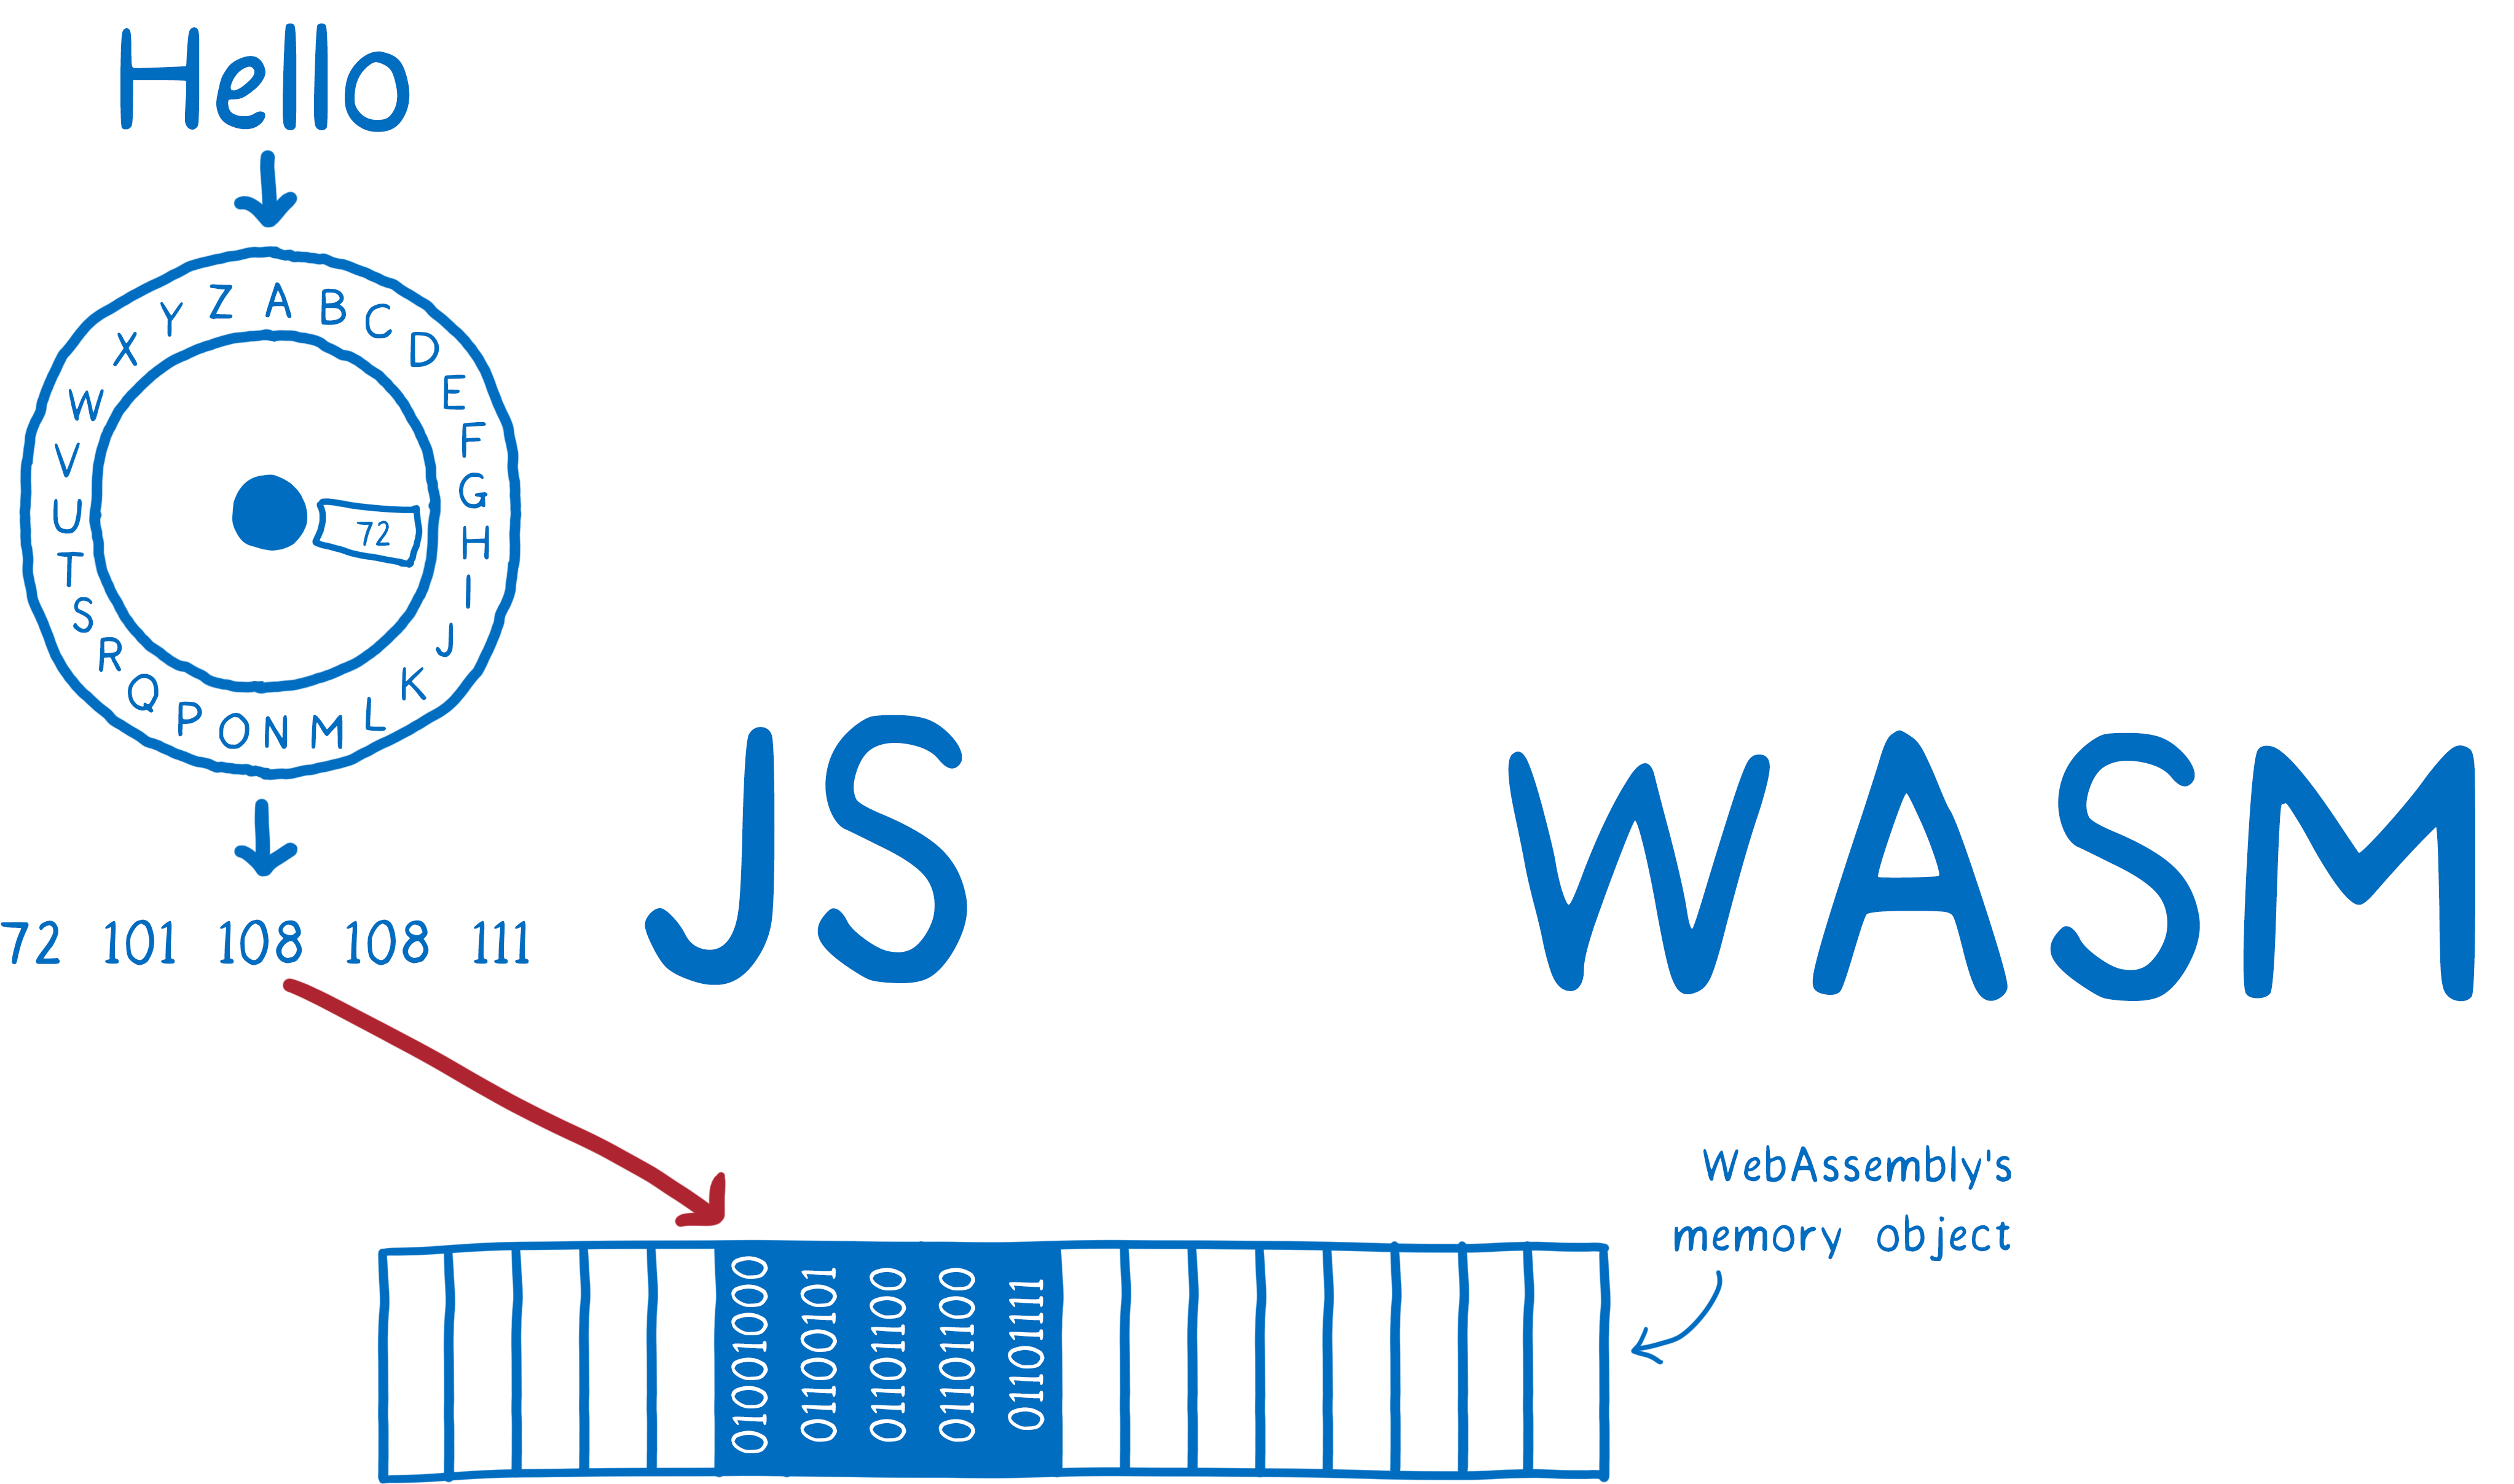
\includegraphics[width=0.5\textwidth]{figures/wasm_bindgen.png}
  \caption{JS string naar wasm conversie}
\end{figure}

\clearpage

Dit betekent dat JS functies vanuit Rust worden aangeroepen met de types die deze functies
verwachten:
\begin{figure}[h]
\begin{minipage}{.5\textwidth}
\begin{minted}{rust}
#[wasm_bindgen]
extern {
  type console;
  #[wasm_bindgen(static = console)]
  fn log(s: &str);
}
\end{minted}
\end{minipage}\hfill
\begin{minipage}{.5\textwidth}
\begin{minted}{rust}
#[wasm_bindgen]
pub fn foo() {
  console::log("hello!");
}


\end{minted}
\end{minipage}
\end{figure}

Of structs gebruiken in Rust en ze laten werken als klassen in JS:

\begin{figure}[h]
\begin{minipage}{.5\textwidth}
\begin{minted}{rust}
// rust
#[wasm_bindgen]
pub struct Foo {
  contents: u32,
}

#[wasm_bindgen]
impl Foo {
  pub fn new() -> Foo {
    Foo { contents: 0 }
}
\end{minted}
\end{minipage}\hfill
\begin{minipage}{.5\textwidth}
\begin{minted}{javascript}
// JS
import {Foo} from "./js_hello_world";

let foo = Foo.new();
assertEq(foo.add(10), 10);
foo.free();





\end{minted}
\end{minipage}
\end{figure}

Na het compileren, zijn er een heleboel bestanden. Om van die bestanden naar een npm package te
gaan, is er de \mintinline{rust}{wasm-pack} library. Het zal \mintinline{rust}{wasm-bindgen} voor je
draaien. Dan, zal het alle bestanden nemen en ze verpakken. Het zal een package.json  er aan
toevoegen, waarin alle npm dependencies van uw Rust code zijn ingevuld. Ten slotte, alles wat je
hoeft te doen is \mintinline{bash}{npm publish}.

\begin{figure}[h]
  \centering
  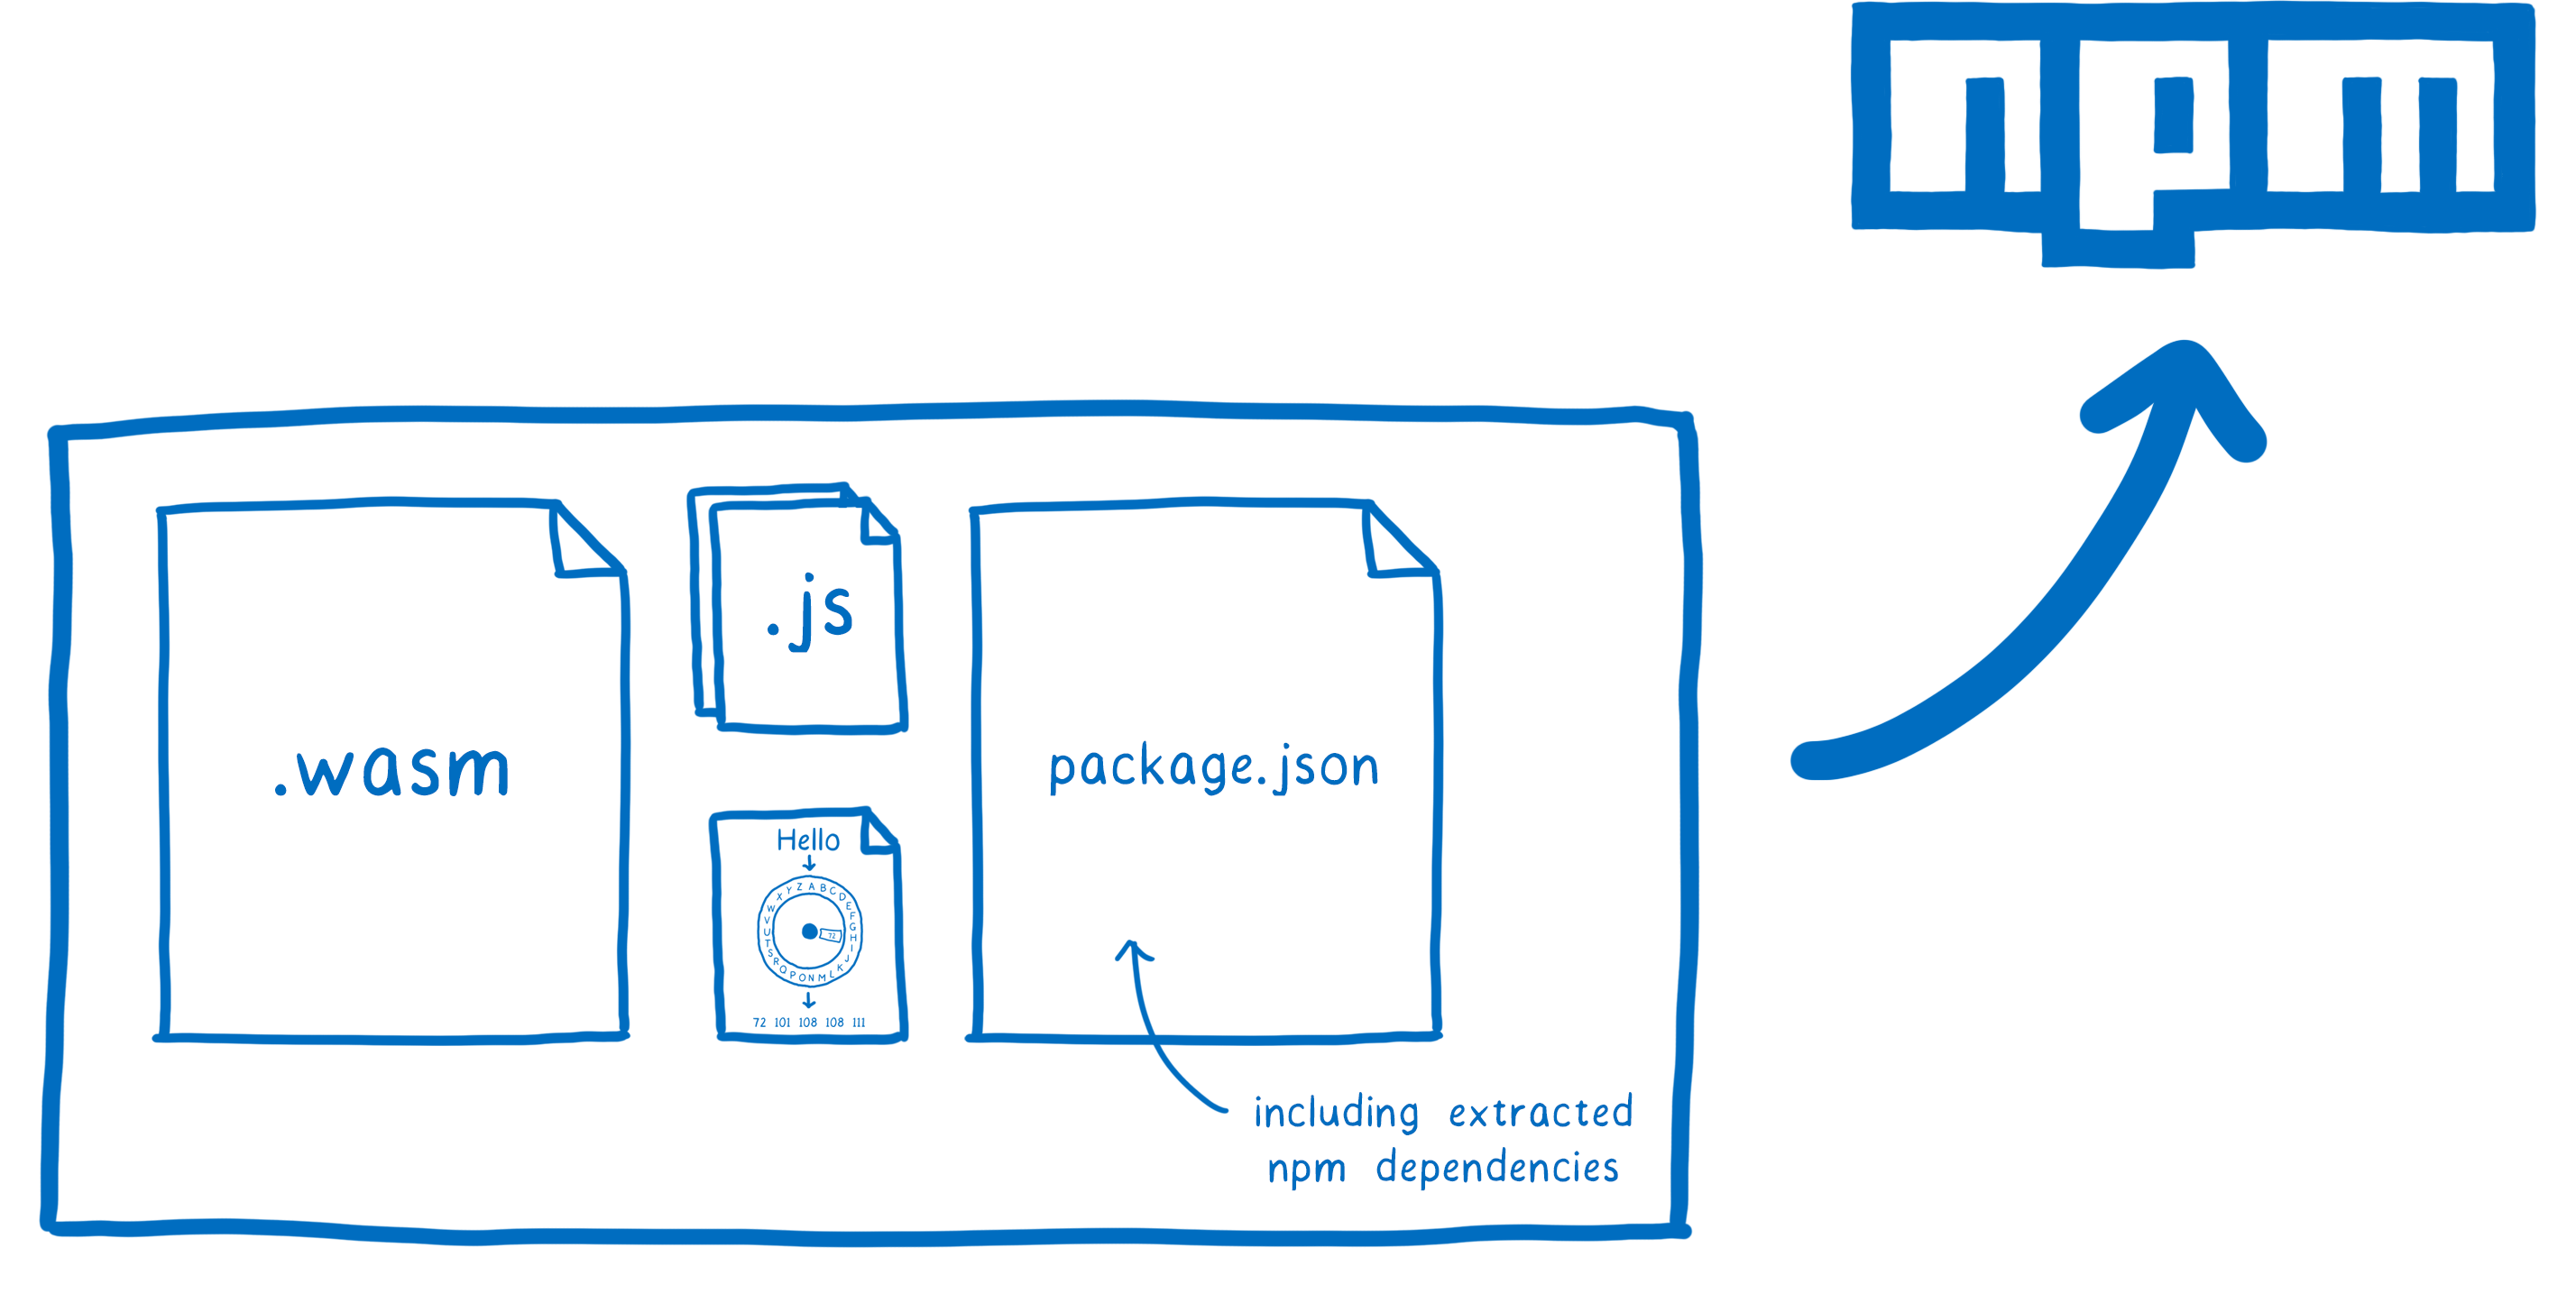
\includegraphics[width=0.7\textwidth]{figures/wasm_to_npm.png}
  \caption{publiceren van wasm als npm package}
\end{figure}




\clearpage

\section{Welke front- \& backend frameworks zijn er ter beschikking?}
\label{frameworks}

Om efficiënt webapplicaties te bouwen heeft u een degelijk framework nodig die voor jou al het zware
werk doet. Gelukkig heeft Rust mits zijn jonge jaren, al een aardig aantal frameworks ter
beschikking voor het bouwen van webapplicaties.  

Dit zijn de top 3 front- en backend frameworks. Gerangschikt naar mate van hun populariteit (GitHub
stars).

\subsection{Frontend}

\subsubsection{Yew - 21k} 

Yew is het populairste frontend framework met over 21k GitHub stars. Het beschikt
over een component-gebaseerd framework dat het makkelijk maakt om interactieve UI’s te maken.
Ontwikkelaars die ervaring hebben met frameworks als React en Elm zouden zich helemaal thuis moeten
voelen bij het gebruik van Yew. Naast de aangename developer experience brengt het ook geweldige
prestaties met zich mee. Dit bereiken ze door het minimaliseren van het aanroepen naar de DOM en
door ontwikkelaars te helpen om gemakkelijk taken te offloaden naar achtergrond threads met behulp
van web workers. 

De documentatie over de huidige release versie 19.0 is uitgebreid geschreven.  Er kan zelfs al
gekeken worden naar de volgende release “Next”, die refereert naar de master branch. In de Next
versie is belangrijkste nieuwe feature SSR, want de huidige versie heeft alleen maar CSR.

\subsubsection{Dixous - 3.8k}

Dixous is een opkomend en jong UI framework als concurrent voor Yew. Het is net als Yew ontworpen om
React-achtig te zijn. Zo heeft het ook een component-gebaseerde architectuur, state management,
props en nog veel meer. Buiten de verschillende syntax tegen over Yew, heeft Dixous nog een aantal
troeven zoals:  
\begin{itemize}
  \item de keuze tussen JSX-achtige of hun eigen macro gebaseerde RSX syntax als templating systeem
    ingebouwde globale state en error handler 

  \item components en hooks kunnen worden hergebruikt voor te renderen op het web, desktop, mobiel,
    server en meer 

  \item uitgebreide inline documentatie 

  \item SSR 
\end{itemize}

\subsubsection{Seed - 3.3k}

Seed is een frontend framework voor het maken van prestatiegerichte en betrouwbare webapps die een
Elm-achtige architectuur heeft. Het heeft een minimale configuratie en boilerplate, en heeft
duidelijke documentatie die het voor iedereen gemakkelijk maakt om mee te beginnen.  

Ook Seed gebruikt een eigen templating systeem met een macro syntax waardoor Rustaceans zich meteen
thuis voelen. Dit betekent dat linting, formatteren en commentaar geven zullen werken, en het is
allemaal in Rust. Dit in tegenstelling tot een JSX-achtige syntax (zoals die van Yew) die
afhankelijk is van IDE-extensies om de developer experience te verbeteren. 

Seed beschikt niet over SSR en heeft nog geen plannen om het te implementeren. 

\subsection{Backend}

\subsubsection{Rocket – 17.2k}

Rocket is een populair webframework dat het voor developers gemakkelijk maakt om snelle webapps te
schrijven zonder te bezuinigen op veiligheid, flexibiliteit of functionaliteiten. Het heeft
ondersteuning voor het testen van libraries, cookies, streams, routes, templates, databases, ORMs,
boilerplates, en nog veel meer. Rocket heeft ook een grote en actieve community. 

\subsubsection{Actix-web – 14.1k}

Net als Rocket, is Actix een ander krachtig backend web framework. Actix heeft een
architectuurpatroon gebaseerd op het actor-systeem van Rust en is goed uitgerust voor het bouwen van
schrijfdiensten en micro apps. Het heeft ondersteuning voor routing, middleware, testen, WebSockets,
automatisch server reloading en kan gehost worden op NGINX. Actix kan worden gebruikt om een
volledige web app en API te bouwen. 

\subsubsection{Axum – 4.7k}

Alhoewel er nog populairdere frameworks zijn dan Axum verdient het zeker een plaats in de top 3.
Axum is deel van het populaire Tokio project, met sponsors als aws, azure en facebook. Tokio is een
asynchrone runtime voor Rust, die de bouwstenen biedt die nodig zijn voor het schrijven van
netwerktoepassingen. 

Axum is een laag bovenop Tokio’s HTTP client genaamd hyper, die een relatief low-level library is en
bedoeld is al bouwsteen voor libraries en applicaties. Het framework focust op ergonomie en
modulariteit. Wat het nog onderscheidt met andere frameworks, is dat het geen eigen middleware
systeem heeft maar gebruikt in plaats daarvan de tower::Service module van het Tokio project. Dit
betekent dat Axum gratis timeouts, tracing, compressie, authorisatie en meer krijgt. 

Dit alles maakt met zijn jonge 1-jarige leeftijd toch een library om naar uit te kijken. 

\clearpage

\section{Hoe bouwt u een webapp in Rust?}

Sinds Yew het populairste framework is en ook is gebruikt als framework voor het bouwen van de speed
typing applicatie, zal de vraag \enquote{Hoe bouwt u een webapp in Rust} beantwoord worden met Yew
als framework. Het bouwen van een webapplicatie in een ander framework zal in grote lijnen hetzelfde
zijn. Dit zal een praktische kijk zijn op hoe we Yew kunnen gebruiken voor het bouwen van
Webapplicaties. \cite{yew_introduction}

In dit voorbeeld gaan we een simpele Todo applicatie bouwen.

\subsection{Tools installeren}

\subsubsection{Rust}
Om Rust te installeren hebben we de rustup toolchain installer nodig. Met het onderstaand script kan
je het installeren op jouw UNIX machine. Als u Rust al hebt staan maak dan zeker dat u de laatste
versie heeft door \mintinline{rust}{rustup update} uit te voeren.

\begin{minted}{bash}
curl --proto '=https' --tlsv1.2 -sSf https://sh.rustup.rs | sh
\end{minted}

\subsubsection{WebAssembly}

Rust kan source codes compileren voor verschillende 'targets' (m.a.w verschillende processors). Het
compilatie target voor een browser gebaseerd WebAssembly heet wasm32-unkown-unkown. Het volgende
commando zal het WebAssembly target toevoegen aan uw development environment.

\begin{minted}{bash}
rustup target add wasm32-unknown-unknown
\end{minted}

\clearpage

\subsubsection{Trunk}

De documentatie van Yew raad aan om Trunk te gebruiken voor het beheren van deployment en packaging.

\begin{minted}{bash}
cargo install --locked trunk
\end{minted}

Nu ons development enviroment opgezet is, kunnen we een nieuw cargo project aanmaken.

\begin{minted}{bash}
cargo new yew-app
cd yew-app
\end{minted}

Om te verifieren dat het Rust environment juist is opgezet, voert u het initiele project uit met de
cargo build tool. Na de output van de het build process, zou u normaal \mintinline{rust}{"Hello,
world!"} te zien
krijgen.

\begin{minted}{bash}
cargo run
\end{minted}

\subsubsection{Statische pagina}

Om deze simpele command line applicatie naar een basis Yew web applicatie te convertern, zijn er een
paar aanpassingen nodig. Pas de volgende bestanden aan als volgt:

\begin{listing}[h]
\begin{minted}{toml}
[package]
name = "yew-app"
version = "0.1.0"
edition = "2021"

[dependencies]
yew = "0.19"
\end{minted}
\caption{Cargo.toml}
\end{listing}

\clearpage

\begin{listing}[h]
\begin{minted}{rust}
use yew::prelude::*;

#[function_component(App)]
fn app() -> Html {
    html! {
        <h1>{ "Hello World" }</h1>
    }
}

fn main() {
    yew::start_app::<App>();
}
\end{minted}
\caption{main.rs}
\end{listing}

Maak nu een index.html aan in de root folder van het project.

\begin{listing}[h]
\begin{minted}{html}
<!DOCTYPE html>
<html lang="en">
  <head> </head>
  <body></body>
</html>
\end{minted}
\caption{index.html}
\end{listing}

\subsubsection{Start de development server}

Voer het volgende commando uit om de applicatie te builden en lokaal te draaien.

\begin{minted}{bash}
trunk serve --open
\end{minted}

\subsection{Statische pagina}

\subsubsection{Bouwen van HTML}

Yew maakt gebruik van de procedurele macro's van Rust en biedt ons een syntax die lijkt op JSX (een
uitbreiding van JavaScript waarmee u HTML-achtige code kunt schrijven in JavaScript) om de opmaak te
maken.

\clearpage

\subsubsection{Converteren van HTML naar Rust}

Aangezien we al een vrij goed idee hebben van hoe onze website eruit zal zien, kunnen we onze
mentale opzet eenvoudig vertalen naar een voorstelling die compatibel is met html!. Als je
eenvoudige HTML kunt schrijven, moet het geen probleem zijn om markeringen in html! te schrijven.
Het is belangrijk op te merken dat de macro op een paar punten verschilt van HTML:
\begin{itemize}
  \item Uitdrukkingen moeten tussen accolades staan (\{ \})
  \item Er mag maar één root node zijn. Als je
    meerdere elementen wilt hebben zonder ze in een container te wikkelen, wordt een lege
    tag/fragment (<> ... </>) gebruikt
  \item Elementen moeten goed worden afgesloten.
\end{itemize}

We willen een layout bouwen die er ongeveer zo uitziet in ruwe HTML:

\begin{minted}{html}
<main>
  <h1>My todo list</h1>
  <ul>
    <li>
      <input type="checkbox" />
      <label>Take dog out for a walk</label>
    </li>
    <input type="checkbox" />
    <label>Feed the cats</label>
    <li>
      <input type="checkbox" />
      <label>Take out the trash</label>
    </li>
    <li>
      <input type="checkbox" />
      <label>Water plants</label>
    </li>
  </ul>
</main>
\end{minted}

\clearpage

Laten we nu deze HTML in html! omzetten. Type (of kopieer/plak) het volgende knipsel in de body van
de app functie, zodat de waarde van html! wordt geretourneerd door de functie.

\begin{listing}[h]
\begin{minted}{rust}
#[function_component]
pub fn App() -> Html {
  html! {
    <main>
      <h1>{ "My todo list" }</h1>
      <ul>
        <li>
          <input type="checkbox"/>
          <label> { "Take dog out for a walk" } </label>
        </li>
          <input type="checkbox"/>
          <label> { "Feed the cats" } </label>
        <li>
          <input type="checkbox"/>
          <label> { "Take out the trash" } </label>
        </li>
        <li>
          <input type="checkbox"/>
          <label> { "Water plants" } </label>
        </li>
      </ul>
    </main>
  }
}
\end{minted}
\caption{app.rs}
\end{listing}

\clearpage

\subsubsection{Components}

Components zijn de bouwstenen van Yew applicaties. Door components te combineren, die weer uit
andere components kunnen worden opgebouwd, bouwen we onze applicatie. Door onze components te
structureren voor herbruikbaarheid en ze generiek te houden, kunnen we ze in meerdere delen van onze
applicatie gebruiken zonder code of logica te hoeven dupliceren.

In feite is de app functie die we tot nu toe hebben gebruikt een component, genaamd
\mintinline{rust}{App}. Het is een 'function component'. Er zijn twee verschillende soorten
componenten in Yew:
\begin{itemize}
  \item Struct Components 
  \item Function Components
\end{itemize}

In dit voorbeeld zullen we function components gebruiken.

Laten we nu onze \mintinline{rust}{App} component opsplitsen in kleinere componenten. We kunnen onze
Todo lijst opspliten in 2 components genaamd \mintinline{rust}{Task} en \mintinline{rust}{TaskList}.

\begin{listing}[h]
\begin{minted}{rust}
#[derive(Properties, Debug, PartialEq)]
pub struct TaskProps {
  pub id: String,
  pub title: String,
  pub completed: bool,
}

#[function_component]
pub fn Task(
  TaskProps {
    id,
    title,
    completed,
  }: &TaskProps,
) -> Html {
  html! {
    <li>
      <input
        type="checkbox"
        id={id.clone()}
        checked={*completed}
      />
      <label
        for={id.clone()}>{title.clone()}
      </label>
    </li>
  }
}
\end{minted}
\caption{task.rs}
\end{listing}

\clearpage

Let op de parameters van onze \mintinline{rust}{Task} function component. Een function component
heeft slechts één argument dat zijn 'props' (kort voor 'properties') definieert. Props worden
gebruikt om gegevens door te geven van een ouder component naar een kind component. In dit geval is
\mintinline{rust}{TaskProps} een \mintinline{rust}{struct} die de props definieert.

\begin{listing}[h]
\begin{minted}{rust}
#[derive(Properties, PartialEq)]
pub struct TaskListProps {
  pub children: Children,
}
#[function_component]
pub fn TaskList(TaskListProps { children }: &TaskListProps) -> Html {
  html! {
    <ul>
      { for children.iter() }
    </ul>
  }
}
\end{minted}
\caption{task\_list.rs}
\end{listing}

Nu kunnen we onze \mintinline{rust}{App} component updaten met onze nieuwe components
\mintinline{rust}{Task} \& \mintinline{rust}{TaskList}.

\begin{listing}[h]
\begin{minted}{rust}
#[function_component]
pub fn App() -> Html {
  let tasks = vec![
    html! { 
      <Task id={"1"} title={"Take dog out for a walk"} completed={true} /> 
    },
    // ... andere tasks
  ];
  html! {
    <main>
      <h1>{ "My todo list" }</h1>
      <TaskList>
        {tasks}
      </TaskList>
    </main>
  }
}
\end{minted}
\caption{app.rs}
\end{listing}

\clearpage

\subsubsection{Interactief}
Momenteel doet onze applicatie niet veel anders dan onze voor gedefineerde lijst te tonen.
Uiteindlijk willen we onze taken uit de todo lijst kunnen schrappen. Om deze interactie te laten
werken zullen we een aantal zaken aanpassen.

Om bij te houden of de gebruiker de taak geschrapt heeft al dan niet, zullen we een
\mintinline{rust}{completed_state} gebruiken met de \mintinline{rust}{use_state} hook. Zo verliezen
we niet de waarde van de variabele \mintinline{rust}{completed_state} mocht het component
re-renderen.

\begin{minted}{rust}
#[function_component]
pub fn Task(
    ...
) -> Html {
    let completed_state = use_state(|| *completed);
    ...
}
\end{minted}

Het volgende is natuurlijk het \mintinline{rust}{onclick} event afhandelen als de gebruiker op het
label of input element klikt. Hiervoor hebben we een \mintinline{rust}{Callback} functie nodig die
onze \mintinline{rust}{completed_state} aanpast naargelang de vorige state. Voor we de
\mintinline{rust}{completed_state} kunnen gebruiken in onze Callback closure functie moeten we die
eerst clonen. De reden hiervoor is het keyword \mintinline{rust}{move} die voor de closure
parameters staat, \mintinline{rust}{move} zorgt
ervoor dat alle references die gebruikt worden in de closure scope hun waarden worden verplaatst
binnen de scope. Dus om te voorkomen dat we onze \mintinline{rust}{completed_state} nergens meer
kunenn gebruiken clonen we eerst de state.

Daarnaast kunnen we ook een css class meegeven met de \mintinline{rust}{classes!} macro van yew, die
conditioneel het html label zal doorstrepen al dan niet.

\clearpage

\begin{listing}
\begin{minted}{rust}
#[function_component]
pub fn Task(
    TaskProps {
        id,
        title,
        completed,
    }: &TaskProps,
) -> Html {
    let completed_state = use_state(|| *completed);

    let onclick = {
        let completed_state = completed_state.clone();

        Callback::from(move |_| {
            if *completed_state {
                completed_state.set(false);
            } else {
                completed_state.set(true);
            }
        })
    };

    let completed_class = {
        if *completed_state {
            "line-through"
        } else {
            ""
        }
    };

    html! {
        <li>
            <input
                {onclick}
                type="checkbox"
                id={id.clone()}
                checked={*completed_state}
            />
            <label
                class={classes!(completed_class)}
                for={id.clone()}>{title.clone()}
            </label>
        </li>
    }
}
\end{minted}
\caption{task.rs}
\end{listing}

\clearpage

\subsubsection{Data extern ophalen}

In de speed typing applicatie komen de code snippets van een API in plaats van hard gecodeerd te
zijn in de frontend. Laten we onze todo lijst ophalen van een externe bron. Hiervoor moeten we de
volgende crates toevoegen:
\begin{itemize}
  \item reqwasm voor het maken van de fetch call.
  \item serde met derive functies Voor het de-serialiseren van het JSON antwoord
  \item wasm-bindgen-futures voor het uitvoeren van Rust Future als een Promise
\end{itemize}

Laten we de dependencies in het Cargo.toml bestand bijwerken:

\begin{minted}{toml}
[dependencies]
yew = { git = "https://github.com/yewstack/yew/", features = ["csr"] }
serde = { version = "1.0", features = ["derive"] }
wasm-bindgen-futures = "0.4"
\end{minted}

Pas de \mintinline{rust}{TaskProps} struct aan om de \mintinline{rust}{Deserialize} trait af te leiden.

\begin{minted}{rust}
#[derive(Properties, Debug, PartialEq, Deserialize)]
pub struct TaskProps {
  pub id: String,
  pub title: String,
  pub completed: bool,
}
\end{minted}

Als laatste stap moeten we onze App component updaten om de fetch request te maken in plaats van
hardcoded data te gebruiken.

Hier gebruiken we de \mintinline{rust}{use_effect_with_deps} hook met lege dependencies als tweede
parameter om de tasks slechts eenmaal op te halen bij de eerste render van het App component. In de
closure gebruiken we \mintinline{rust}{wasm-bindgen-futures} om de Javascript Promise die de
\mintinline{rust}{Request::get} genereert om te zetten naar een Future type. Met de
\mintinline{rust}{Request::get} halen we de JSON todos op en slaan ze op als een
\mintinline{rust}{vec} met \mintinline{rust}{TaskProps}. Vervolgens vullen we onze
\mintinline{rust}{tasks} state met de \mintinline{rust}{fetched_tasks} en zullen de tasks worden
weergeven in de browser!

\begin{listing}
\begin{minted}{rust}
#[function_component]
pub fn App() -> Html {
let tasks = use_state(std::vec::Vec::new);
  {
    let tasks = tasks.clone();
    use_effect_with_deps(move |_| {
      wasm_bindgen_futures::spawn_local(async move {
        let fetched_tasks: Vec<TaskProps> = Request::get("url")
          .send()
          .await
          .unwrap()
          .json()
          .await
          .unwrap();

        tasks.set(fetched_tasks.iter().take(10).map(|props| {
            html! { 
              <Task 
                id={props.id.clone()} 
                title={props.title.clone()} 
                completed={props.completed} 
              /> 
            }
          }).collect()
        );
      });
      || ()
    }, ());
  }

  html! {
      <main>
          <h1>{ "My todo list" }</h1>
          <TaskList>
              { (*tasks).clone() }
          </TaskList>
      </main>
  }
}
\end{minted}
\caption{app.rs}
\end{listing}

\clearpage

\section{Hoe bouwt u een API in Rust?}

Volgend op de Todo applicatie die we gebouwd hebben in \enquote{Hoe bouwt u een webapp in Rust?},
zullen we een REST API bouwen die de taken uit een database zal halen en opslaan. Als API framework
zullen we Actix-web gebruiken, samen met diesel.rs als ORM voor het beheren van de database. Om het
simpel te houden gebruiken we net zoals in de speed typing test applicatie SQLite als database.
\cite{diesel} \cite{actix_docs}


\subsection{Opzet project}

Maak een nieuw Rust project aan met de volgende dependencies.

\begin{minted}{bash}
cargo new api
cd api/
\end{minted}

\begin{listing}[h]
\begin{minted}{toml}
[dependencies]
diesel = { version = "1.4.8", features = ["sqlite", "r2d2"] }
dotenv = "0.15.0"
actix-web = "4"
actix-cors = "0.6.1"
uuid = { version = "0.8", features = ["serde", "v4"] }
serde = { version = "1.0", features = ["derive"] }
serde_json = "1.0"
log = "0.4"
env_logger = "0.9.0"
\end{minted}
\caption{Cargo.toml}
\end{listing}

We zullen uitleggen waarom we deze dependencies nodig hebben als we verder gaan.

\subsubsection{Database}

Diesel biedt een aparte CLI tool om uw project te helpen beheren. Omdat het een standalone binary
is, en geen directe invloed heeft op de code van uw project, voegen we het niet toe aan Cargo.toml.
In plaats daarvan installeren we het gewoon op ons systeem.

\begin{minted}{bash}
echo DATABASE_URL=todo.db > .env
\end{minted}

Nu kan Diesel CLI alles voor ons opzetten.

\begin{minted}{bash}
diesel setup
\end{minted}

Dit zal onze database aanmaken (als die nog niet bestond), en een lege migrations directory aanmaken
die we kunnen gebruiken om ons schema te beheren.

Diesel support momenteel alleen een database-first aanpak. Hierbij maken we eerst het database
schema om dan met migrations het schema naar Rust om te zetten. Dat gezegd zijnde, laat ons een
eerste migration aanmaken.

\begin{minted}{bash}
diesel migration generate create_tasks
\end{minted}

Diesel CLI zal twee lege bestanden (\mintinline{rust}{up.sql} en \mintinline{rust}{down.sql}) voor
ons aanmaken in de vereiste structuur. In deze bestanden schrijven we SQL voor de Task tabel aan te
maken in \mintinline{rust}{up.sql} en als we de migration willen ongedaan maken in
\mintinline{rust}{down.sql}.

\begin{listing}
\begin{minted}{sql}
CREATE TABLE tasks (
  id VARCHAR NOT NULL PRIMARY KEY,
  title VARCHAR NOT NULL,
  completed INTEGER NOT NULL DEFAULT 0
)
\end{minted}
\caption{up.sql}
\end{listing}

\begin{listing}
\begin{minted}{sql}
DROP TABLE tasks
\end{minted}
\caption{down.sql}
\end{listing}

Nu kunnen we onze eerste migration uitvoeren met:

\begin{minted}{bash}
diesel migration run
\end{minted}

Dit zal onze SQL migration uitvoeren op de \mintinline{bash}{todo.db} database en het nodige Rust
schema genereren met de nodige types. In het Rust schema wordt met de \mintinline{rust}{table!}
macro een hoop code gegeneerd gebaseerd op het database schema om alle tabellen en kolommen weer te
geven. Zo kunnen we nu gebruik maken van Rust zijn krachtig typesysteem om volledige SQL queries te
gaan bouwen met code. We zullen in het volgende voorbeeld zien hoe we dat precies kunnen gebruiken.

Telkens wanneer we een migratie uitvoeren of terugdraaien, wordt dit bestand automatisch bijgewerkt.

\clearpage

\subsection{API}

Om de basis functionaliteiten van onze Todo applicatie in de front-end te ondersteunen, zal onze API
een nieuwe taak kunnen aanmaken en de lijst met taken ophalen. Dus zullen we de volgende endpoints
hebben:
\begin{itemize}
  \item GET /tasks - retourneert alle taken
  \item POST /tasks - voegt een nieuwe taak toe
\end{itemize}


Om onze code overzichtelijklijk te houden, zullen we de volgende structuur hanteren:
\dirtree{%
.1 src/.
.2 main.rs.
.2 models.rs.
.2 schema.rs.
.2 handlers.rs.
.2 db.rs.
}

Bij het opzetten van ons project heeft cargo een al een \mintinline{bash}{main.rs} bestand
aangemaakt. Laten we dat bewerken en onze eerste \mintinline{rust}{"Hello World!"} route schrijven.

\begin{listing}[h]
\begin{minted}{rust}
use actix_web::{web, App, HttpServer};

#[actix_web::main]
async fn main() -> std::io::Result<()> {
  HttpServer::new(|| {
    App::new()
      .route("/hello", web::get().to(|| async { "Hello World!" }))
  })
  .bind(("127.0.0.1", 5000))?
  .run()
  .await
}
\end{minted}
\caption{main.rs}
\end{listing}
\clearpage

Onze main functie heeft nu het \mintinline{rust}{#[actix_web::main]} attribuut, die zal onze main
functie markeren als start functie en uitvoeren in de runtime van \mintinline{rust}{actix_web}.

Een belangrijk punt om op te merken is dat we een \mintinline{rust}{Result} type teruggeven. Dit
stelt ons in staat om de \mintinline{rust}{?} operator in main te gebruiken, die elke fout die door
de geassocieerde functie wordt teruggegeven naar de aanroeper koppelt.

Het tweede ding om op te merken is \mintinline{rust}{async/await}. Hiermee geven we aan dat Rust
onze functies asynchroon kan uitvoeren zonder andere threads te blokkeren.

In onze main, instantiëren we een \mintinline{rust}{HttpServer}, voegen er een
\mintinline{rust}{App} aan toe die dient als een
Application factory en voegen onze eerste route er aan toe.

Als alles goed gaat zou u nu de API kunnen opstarten met \mintinline{bash}{cargo run} en bij een
GET request naar \mintinline{bash}{localhost:8080/hello} \mintinline{rust}{"Hello world!"} als repons 
te zien krijgen.

\begin{listing}[h]
\begin{minted}{rust}
#[get("/task")]
async fn get_tasks() -> Result<HttpResponse, Error> {
  todo!()
}

#[post("/task")]
async fn add_task() -> Result<HttpResponse, Error> {
  todo!()
}
\end{minted}
\caption{handlers.rs}
\end{listing}

In de module \mintinline{rust}{handlers} zullen we onze requests per endpoint afhandelen. Voorlopig
gebruiken we hier nog de \mintinline{rust}{todo}! macro sinds we nog geen communicatie maken de
database. Laat ons dat eerst aanpakken.

Onze eerste migration die we eerder hebben uitgevoerd heeft voor ons al een
\mintinline{rust}{schema.rs} module aangemaakt, zodat diesel onze queries kan controleren tijdens
het compileren. Om met queries te kunnen werken in Rust hebben we models nodig. Zo kunnen we het
resultaat van een query mappen naar een model of een model gebruiken voor nieuwe data in te voegen.

Met de traits \mintinline{rust}{Queryable} en \mintinline{rust}{Insertable} zorgen we er voor dat de
struct \mintinline{rust}{Task} als resultaat voor een query kan gebruikt worden en als struct om
nieuwe data in te voegen.

\mintinline{rust}{Deserialize} en \mintinline{rust}{Serialize} komen van de crate
\mintinline{rust}{serde}, zij zorgen ervoor dat we de models kunnen omzetten naar json en andersom.

\clearpage

\begin{listing}[h]
\begin{minted}{rust}
#[derive(Debug, Serialize, Deserialize, Queryable, Insertable)]
pub struct Task {
  pub id: String,
  pub title: String,
  pub completed: bool,
}

#[derive(Debug, Serialize, Deserialize)]
pub struct InputTask {
  pub title: String,
}
\end{minted}
\caption{models.rs}
\end{listing}

Nu we onze models hebben kunnen we in \mintinline{rust}{db} functies schrijven om tasks op te vragen
en aan te maken. De functies spreken voorzich, we gebruiken diesel zijn sql implementaties om met
onze database te communiceren.

Merk op dat we bij elke functie \mintinline{rust}{schema::tasks::dsl::*} opnieuw toevoegen aan de
lokale scope. Dit is puur conventie sinds we maar 1 tabel hebben \mintinline{rust}{Tasks}, moesten
we meerdere tabellen hebben zouden we onze scope kunnen vervuilen door bijvoorbeeld zelfde
kolomnamen die elkaar overschrijven.

\begin{listing}[h]
\begin{minted}{rust}
type DbError = Box<dyn std::error::Error + Send + Sync>;

pub fn list_all_tasks(conn: &SqliteConnection) 
  -> Result<Option<Vec<Task>>, DbError> {
  use crate::schema::tasks::dsl::*;
  Ok(tasks.load::<Task>(conn).optional()?)
}
pub fn insert_new_task(t: &str, conn: &SqliteConnection) 
  -> Result<Task, DbError> {
  use crate::schema::tasks::dsl::*;
  let new_task = Task {
    id: Uuid::new_v4().to_string(),
    title: t.to_owned(),
    completed: false,
  };
  diesel::insert_into(tasks).values(&new_task).execute(conn)?;
  Ok(new_task)
}
\end{minted}
\caption{db.rs}
\end{listing}

\clearpage

Nu we onze helper functies geschreven hebben kunnen we de requests afhandelen in
\mintinline{rust}{handlers} als volgt:

Elke handler functie krijgt een connection pool als parameter, die we later zullen definieren in
main. De connection pool zal verschillende connecties met de database openhouden zodat ze efficient
kunnen hergebruikt worden door anderen. Om te voorkomen dat een andere thread de connectie gebruikt
tijdens het uitvoeren van een \mintinline{rust}{db} functie blokkeren we deze thread met
\mintinline{rust}{web::block}. Als alles goed verloopt geven we de resultaten terug, indien niet
geven we een \mintinline{rust}{InternalServerError} terug.

\begin{listing}[h]
\begin{minted}{rust}
#[get("/task")]
async fn get_tasks(
  pool: web::Data<DbPool>,
) -> Result<HttpResponse, Error> {
  let tasks = web::block(move || {
    let conn = pool.get()?;
    db::list_all_tasks(&conn)
  })
  .await?
  .map_err(actix_web::error::ErrorInternalServerError)?;

  if let Some(tasks) = tasks {
    Ok(HttpResponse::Ok().json(tasks))
  } else {
    let res = HttpResponse::NotFound().body("No tasks found!".to_string());
    Ok(res)
  }
}
#[post("/task")]
async fn add_task(
  pool: web::Data<DbPool>,
  form: web::Json<models::InputTask>,
) -> Result<HttpResponse, Error> {
  let task = web::block(move || {
    let conn = pool.get()?;
    db::insert_new_task(&form.title, &conn)
  })
  .await?
  .map_err(actix_web::error::ErrorInternalServerError)?;

  Ok(HttpResponse::Created().json(task))
}
\end{minted}
\caption{handler.rs}
\end{listing}

\clearpage

Wat ons nu nog rest te doen, is onze connection pool instantiëren en de handler functies linken aan
onze App. Vooraleer dat we dat doen laden we eerst ons .env bestand in het enviroment met de
\mintinline{rust}{dotenv} crate en loggen we info over de applicatie naar \mintinline{bash}{stdout}
met \mintinline{rust}{env_logger}. Daarna kunnen we onze connection pool opzetten met de
\mintinline{bash}{DATABASE_URL} uit het enviroment. Ten slotte voegen we onze hanlder functies toe
aan een nieuwe service met als scope \mintinline{bash}{/api} zodat al onze routes worden ge prefixed
met \mintinline{bash}{/api}.

\begin{listing}[h]
\begin{minted}{rust}
type DbPool = r2d2::Pool<ConnectionManager<SqliteConnection>>;
#[actix_web::main]
async fn main() -> std::io::Result<()> {
  dotenv::dotenv().ok();
  env_logger::init_from_env(
    env_logger::Env::new().default_filter_or("info")
  );
  // set up database connection pool
  let conn_spec = std::env::var("DATABASE_URL").expect("DATABASE_URL");
  let manager = ConnectionManager::<SqliteConnection>::new(conn_spec);
  let pool = r2d2::Pool::builder()
    .build(manager)
    .expect("Failed to create pool.");
  log::info!(
    "{}",
    format!("starting HTTP server at http://localhost:5000"
  ));
  // Start HTTP server
  HttpServer::new(move || {
    App::new()
      .app_data(web::Data::new(pool.clone()))
      .wrap(middleware::Logger::default())
      .service(
        web::scope("/api")
        .service(get_tasks)
        .service(add_task)
      )
    })
  .bind(("127.0.0.1", 5000))?
  .run()
  .await
}
\end{minted}
\caption{main.rs}
\end{listing}


\clearpage

\section{Is Rust productie klaar?}
\label{productie}

Wanneer een taal 'productie klaar' benoemd kan worden is eigenlijk een moeilijke vraag om te
beantwoorden. Wat 'productie klaar' betekent hangt af van verschillende factoren voor een specifiek
domein. Rust schittert bijvoorbeeld in productief veilige en performante applicaties te bouwen. Top
bedrijven zoals Amazon, Facebook, Microsoft kunnen dit beamen sinds ze ondertussen al een aantal jaar
Rust gebruiken \cite{rust_companies}. Zo heeft Amazon in 2018 Firecracker gelanceerd
\cite{aws_sustainability}. Een open source virtualisatietechnologie die AWS Lambda en andere
serverloze aanbiedingen aandrijft. Daarnaast gebruiken ze Rust ook voor services te leveren zoals
Amazon Simple Storage Service (Amazon S3), Amazon Elastic Compute Cloud (Amazon EC2), Amazon
CloudFront, en meer. Amazon heeft dan ook samen met Google, Microsoft, Huawei en Mozilla de Rust
foundation opgericht in 2020, met een missie om het ontwikkelen van Rust te ondersteunen. We kunnen
dus concluderen dat de taal op zich wel een stabiele omgeving is. Dit onderzoek gaat natuurlijk wel
over hoe we Rust kunnen gebruiken voor het bouwen van webapplicaties. We richten onze focus dan ook
op dit domein. We zullen de deelvraag “Is Rust productie klaar?” opsplitsen in twee delen namelijk
frontend en backend. 

\subsection{Backend }

Laten we beginnen met de backend. Bij het bouwen van hedendaagse webapplicaties heeft u over het
algemeen 2 zaken nodig, een API en een database. Uiteraard is dit niet altijd het geval maar laten
we onze focus hierop leggen. 

Om een web API te bouwen gebruikt u gewoonlijk een web framework. Het huidige rust ecosysteem heeft
een aantal stabiele web frameworks ter beschikking. Uit de deelvraag “Hoe bouwt u een API in
Rust?” hebben we gekozen voor Actix-web te gebruiken als framework. Actix-web voorziet alles wat je
kan verwachten van een web framework, van routing en middleware, tot templating en JSON/form
afhandeling. Het is ook een van de snelste web frameworks ter beschikking. Zo staat actix momenteel
op de 5de plaats bij een benchmark ranking van alle populaire web frameworks (ook andere
programmeertalen dan Rust) \cite{web_bench}. 

Het actix framework ondersteunt verschillende soorten databases zoals mongodb, postgres, redis,
sqlite, graphql, elasticsearch en meer. De ene database heeft meer ondersteuning dan de andere, maar
naarmate de tijd vordert zal de ondersteuning alleen maar verbeteren. 

\subsection{Frontend}

Bij de frontend komt er wat meer bij kijken. Er zijn namelijk twee opties waarvoor Rust gebruikt kan
worden: 
\begin{itemize}
  \item Een gedeelde in Rust schrijven en compileren naar wasm om vervolgens te importeren als een node
    module in een bestaande Javascript applicatie. 
  \item Een volledige frontend in Rust schrijven met een web framework als Yew en compileren naar wasm 
\end{itemize}               

\clearpage

De eerste optie is meteen ook de optie waarvoor wasm het meest zal gebruikt worden. Zo kan je
bijvoorbeeld Javascript gebruiken voor de UI en wasm voor de logica van de applicatie. Om mogelijks
meer performatie te winnen en correctere code te schrijven. Deze optie wordt al volop in productie
gebruikt door meerdere bedrijven \cite{made_with_wasm}: 
\begin{itemize}
  \item 1Password – gebruikt wasm om hun browser plugin te versnellen 
  \item Figma – gebruikt wasm om hun originele C++ applicatie te exporteren naar de browser 
  \item SketchUp – gebruikt wasm om een 3d modelling tool op het web te draaien, wat snelle en
    voorspelbare prestaties verreist 
\end{itemize}

De andere optie, een volledige frontend bouwen met Rust, is een optie die momenteel meer gebruikt
wordt voor hobby projecten dan voor productie. Een van de redenen hiervoor is dat het ecosysteem nog
zeer jong is. Het is bijvoorbeeld niet te vergelijken met het ecosysteem van populaire JS
frameworks, wat ook logisch is. Desondanks het ecosysteem wordt Yew aan een snel tempo ontwikkeld.
Waar sommige libraries als React jaren over doen om features uit te brengen als SSR doet Yew in
enkele maanden.

Het is ook merkwaardig dat Yew degelijk scoort op benchmarks. Natuurlijk presteert Yew beter dan
Javascript frameworks in het werken met geheugen, maar wat vooral opvalt is dat het ook redelijk
presteert in het aanpassen van de DOM. Dit is nu nog een struikel punt voor WebAssembly in het
algemeen, sinds er nog altijd javascript functies worden gebruikt voor het aanpassen van de DOM.
Dat is een van de redenen waarom we hogere bundel grootes over het netwerk zien bij Yew.
Een andere reden is dat WebAssembly zelf niet beschikt over geheugen beheer en garbage collectors.
Om die reden wordt vaak een runtime meegeleverd met de logica van uw applicatie. In sommige gevallen
(Rust) is deze runtime vrij licht, en in andere (Blazor) is het zeer zwaar. We zullen waarschijnlijk
zien dat het gewicht van deze runtimes in de loop van de tijd aanzienlijk zal afnemen door nieuwe
WebAssembly mogelijkheden (garbage collection, module caching) en betere compilatietechnieken
(ahead-of-time compilation).

De resultaten van de benchmarks zijn terug te vinden in Bijlage \ref{appendix:bench}. Let wel op de
bundle grootte van Yew is nog niet geoptimaliseert, met optimalisaties is het mogelijk om de bundle
grootte naar $\sim$100kB te krijgen.

\subsection{Conclusie}

Om Rust in productie te gebruiken kan dus zeker. De vraag is alleen of dit enige meerwaarden heeft
voor het bedrijf. Het antwoord hierop is terug te vinden Hoofdstuk \ref{reflectie} reflectie waar
de vraag wordt afgetoetst met mensen uit de praktijk.
